\documentclass[]{article}
\usepackage{lmodern}
\usepackage{amssymb,amsmath}
\usepackage{ifxetex,ifluatex}
\usepackage{fixltx2e} % provides \textsubscript
\ifnum 0\ifxetex 1\fi\ifluatex 1\fi=0 % if pdftex
  \usepackage[T1]{fontenc}
  \usepackage[utf8]{inputenc}
\else % if luatex or xelatex
  \ifxetex
    \usepackage{mathspec}
  \else
    \usepackage{fontspec}
  \fi
  \defaultfontfeatures{Ligatures=TeX,Scale=MatchLowercase}
\fi
% use upquote if available, for straight quotes in verbatim environments
\IfFileExists{upquote.sty}{\usepackage{upquote}}{}
% use microtype if available
\IfFileExists{microtype.sty}{%
\usepackage{microtype}
\UseMicrotypeSet[protrusion]{basicmath} % disable protrusion for tt fonts
}{}
\usepackage[margin=1in]{geometry}
\usepackage{hyperref}
\hypersetup{unicode=true,
            pdftitle={An Introduction to Discrete Choice Analysis in R},
            pdfauthor={Robert Hickman},
            pdfborder={0 0 0},
            breaklinks=true}
\urlstyle{same}  % don't use monospace font for urls
\usepackage{color}
\usepackage{fancyvrb}
\newcommand{\VerbBar}{|}
\newcommand{\VERB}{\Verb[commandchars=\\\{\}]}
\DefineVerbatimEnvironment{Highlighting}{Verbatim}{commandchars=\\\{\}}
% Add ',fontsize=\small' for more characters per line
\usepackage{framed}
\definecolor{shadecolor}{RGB}{248,248,248}
\newenvironment{Shaded}{\begin{snugshade}}{\end{snugshade}}
\newcommand{\KeywordTok}[1]{\textcolor[rgb]{0.13,0.29,0.53}{\textbf{#1}}}
\newcommand{\DataTypeTok}[1]{\textcolor[rgb]{0.13,0.29,0.53}{#1}}
\newcommand{\DecValTok}[1]{\textcolor[rgb]{0.00,0.00,0.81}{#1}}
\newcommand{\BaseNTok}[1]{\textcolor[rgb]{0.00,0.00,0.81}{#1}}
\newcommand{\FloatTok}[1]{\textcolor[rgb]{0.00,0.00,0.81}{#1}}
\newcommand{\ConstantTok}[1]{\textcolor[rgb]{0.00,0.00,0.00}{#1}}
\newcommand{\CharTok}[1]{\textcolor[rgb]{0.31,0.60,0.02}{#1}}
\newcommand{\SpecialCharTok}[1]{\textcolor[rgb]{0.00,0.00,0.00}{#1}}
\newcommand{\StringTok}[1]{\textcolor[rgb]{0.31,0.60,0.02}{#1}}
\newcommand{\VerbatimStringTok}[1]{\textcolor[rgb]{0.31,0.60,0.02}{#1}}
\newcommand{\SpecialStringTok}[1]{\textcolor[rgb]{0.31,0.60,0.02}{#1}}
\newcommand{\ImportTok}[1]{#1}
\newcommand{\CommentTok}[1]{\textcolor[rgb]{0.56,0.35,0.01}{\textit{#1}}}
\newcommand{\DocumentationTok}[1]{\textcolor[rgb]{0.56,0.35,0.01}{\textbf{\textit{#1}}}}
\newcommand{\AnnotationTok}[1]{\textcolor[rgb]{0.56,0.35,0.01}{\textbf{\textit{#1}}}}
\newcommand{\CommentVarTok}[1]{\textcolor[rgb]{0.56,0.35,0.01}{\textbf{\textit{#1}}}}
\newcommand{\OtherTok}[1]{\textcolor[rgb]{0.56,0.35,0.01}{#1}}
\newcommand{\FunctionTok}[1]{\textcolor[rgb]{0.00,0.00,0.00}{#1}}
\newcommand{\VariableTok}[1]{\textcolor[rgb]{0.00,0.00,0.00}{#1}}
\newcommand{\ControlFlowTok}[1]{\textcolor[rgb]{0.13,0.29,0.53}{\textbf{#1}}}
\newcommand{\OperatorTok}[1]{\textcolor[rgb]{0.81,0.36,0.00}{\textbf{#1}}}
\newcommand{\BuiltInTok}[1]{#1}
\newcommand{\ExtensionTok}[1]{#1}
\newcommand{\PreprocessorTok}[1]{\textcolor[rgb]{0.56,0.35,0.01}{\textit{#1}}}
\newcommand{\AttributeTok}[1]{\textcolor[rgb]{0.77,0.63,0.00}{#1}}
\newcommand{\RegionMarkerTok}[1]{#1}
\newcommand{\InformationTok}[1]{\textcolor[rgb]{0.56,0.35,0.01}{\textbf{\textit{#1}}}}
\newcommand{\WarningTok}[1]{\textcolor[rgb]{0.56,0.35,0.01}{\textbf{\textit{#1}}}}
\newcommand{\AlertTok}[1]{\textcolor[rgb]{0.94,0.16,0.16}{#1}}
\newcommand{\ErrorTok}[1]{\textcolor[rgb]{0.64,0.00,0.00}{\textbf{#1}}}
\newcommand{\NormalTok}[1]{#1}
\usepackage{graphicx,grffile}
\makeatletter
\def\maxwidth{\ifdim\Gin@nat@width>\linewidth\linewidth\else\Gin@nat@width\fi}
\def\maxheight{\ifdim\Gin@nat@height>\textheight\textheight\else\Gin@nat@height\fi}
\makeatother
% Scale images if necessary, so that they will not overflow the page
% margins by default, and it is still possible to overwrite the defaults
% using explicit options in \includegraphics[width, height, ...]{}
\setkeys{Gin}{width=\maxwidth,height=\maxheight,keepaspectratio}
\IfFileExists{parskip.sty}{%
\usepackage{parskip}
}{% else
\setlength{\parindent}{0pt}
\setlength{\parskip}{6pt plus 2pt minus 1pt}
}
\setlength{\emergencystretch}{3em}  % prevent overfull lines
\providecommand{\tightlist}{%
  \setlength{\itemsep}{0pt}\setlength{\parskip}{0pt}}
\setcounter{secnumdepth}{0}
% Redefines (sub)paragraphs to behave more like sections
\ifx\paragraph\undefined\else
\let\oldparagraph\paragraph
\renewcommand{\paragraph}[1]{\oldparagraph{#1}\mbox{}}
\fi
\ifx\subparagraph\undefined\else
\let\oldsubparagraph\subparagraph
\renewcommand{\subparagraph}[1]{\oldsubparagraph{#1}\mbox{}}
\fi

%%% Use protect on footnotes to avoid problems with footnotes in titles
\let\rmarkdownfootnote\footnote%
\def\footnote{\protect\rmarkdownfootnote}

%%% Change title format to be more compact
\usepackage{titling}

% Create subtitle command for use in maketitle
\newcommand{\subtitle}[1]{
  \posttitle{
    \begin{center}\large#1\end{center}
    }
}

\setlength{\droptitle}{-2em}

  \title{An Introduction to Discrete Choice Analysis in R}
    \pretitle{\vspace{\droptitle}\centering\huge}
  \posttitle{\par}
    \author{Robert Hickman}
    \preauthor{\centering\large\emph}
  \postauthor{\par}
      \predate{\centering\large\emph}
  \postdate{\par}
    \date{2019-04-24}


\begin{document}
\maketitle

When studying why people make the economic choices they do, we need some
way of quanitfying the value to the person of the offered choices. For
instance, when deciding whether to ride to my office by bike or instead
catch the bus, there are myriad factors that my brain feeds into an
equation to get two values:

\begin{itemize}
\tightlist
\item
  the utility of taking the bus
\item
  the utility of riding my bike
\end{itemize}

For instance, if it looks like it might rain, I'm more likely to take
the bus as getting soaked reduces the utility of cycling to work.
Conversely, if I glance at my watch and see that I've just missed a bus,
the utility of taking the bus decreases as I don't want to have to wait
at the bus stop.

A frquent criticism of economics is that it assumes some \emph{homo
economicus} who will always choose that which maximises this utility.
Lets say the utilities of the two commute choices were onyl governed by
p(rain) and e(wait time) respectively, then for a set probability of
rain and expected wait time for the bus, I should always choose the same
mode of transport. This is clearly not how humans (or any other animal)
work and so for the last 50 years
\href{https://eml.berkeley.edu/~mcfadden/discrete/ch5.pdf}{models of
probabilistic choice} have been used instead.

The advantage to this is that by studying the \% of times I decide to
ride my bike into work vs catching the bus, for any set of parameters,
it's possible to derive the relative utility of that method of
transportation. Then if a novel combination of rain/waiting comes up,
it's possible to predict the chance I will choose to ride my bike and
the chance I will take the bus.

However, many of these models are fairly dense to approach without
formal economic training, so I wanted to write a guide to deriving and
using them in R. For the first post, I'll consider a toy problem with a
simple binary choice paradigm to get some of the basic ideas of random
utility modelling down and progress from there

\section{Example Problem}\label{example-problem}

Summer is here and it's time for the annual Behavioural Economics
departmental picnic! Due to the collapsing global climate, this year is
the hottest yet and you are eagerly anticipating sitting in
\href{https://en.wikipedia.org/wiki/Grantchester_Meadows}{Granchester
Meadows} with your favourite chilled soft drink and discussing your
research.

Unfortuantely, you've been stuck in the office for most of the afternoon
coding up your latest model and will arrive late. Due to the hot
weather, most of the drinks have already been consumed and what's left
needs to be rationed. Luckily, you are all very rational behavioural
economists who know that if you can find everyone's utility for the two
remainnig drinks flavours, you can apportion them appropriately.

The two remaining drinks are
\href{https://media2.giphy.com/media/3oriffxcqE2syOd5Ty/giphy.gif}{buzz
cola} which comes in cans of 330ml which is very tasy, and
\href{https://comb.io/qbzoUv.gif}{slurm} which comes in 2 litre bottles
(which can be poured into any amount).

Someone quickly codes up a binary choice task where PhD students have to
choose between 1,2, or 3 330ml cans of the desirable Buzz Cola, or some
amount between 0 and 2000ml of the slightly less valued Slurm.

Having spent 10 minutes and 1800 trials doing the task your data looks
like

\begin{Shaded}
\begin{Highlighting}[]
\CommentTok{#show the first ten trials}
\KeywordTok{head}\NormalTok{(trial_data, }\DecValTok{10}\NormalTok{)}
\end{Highlighting}
\end{Shaded}

\begin{verbatim}
##      buzz_cola slurm    choice
## 1446         3   800 buzz_cola
## 227          1   800     slurm
## 209          1   800 buzz_cola
## 1497         3   800 buzz_cola
## 1542         3  1200 buzz_cola
## 34           1     0 buzz_cola
## 1493         3   800 buzz_cola
## 1028         2  1600     slurm
## 656          2     0 buzz_cola
## 266          1   800     slurm
\end{verbatim}

If we group by each combination of n(buzz cola cans),ml(slurm) we can
work out the proportion of buzz cola choices

\begin{Shaded}
\begin{Highlighting}[]
\NormalTok{choice_data <-}\StringTok{ }\NormalTok{trial_data }\OperatorTok
\StringTok{  }\CommentTok{#code a buzz cola choice as a binary variable}
\StringTok{  }\KeywordTok{mutate}\NormalTok{(}\DataTypeTok{buzz_cola_choice =} \KeywordTok{case_when}\NormalTok{(}
\NormalTok{    choice }\OperatorTok{==}\StringTok{ "buzz_cola"} \OperatorTok{~}\StringTok{ }\DecValTok{1}\NormalTok{,}
\NormalTok{    choice }\OperatorTok{==}\StringTok{ "slurm"} \OperatorTok{~}\StringTok{ }\DecValTok{0}
\NormalTok{  )) }\OperatorTok
\StringTok{  }\CommentTok{#group by combinations and find the proportion of buzz cola choices}
\StringTok{  }\KeywordTok{group_by}\NormalTok{(buzz_cola, slurm) }\OperatorTok
\StringTok{  }\KeywordTok{summarise}\NormalTok{(}\DataTypeTok{fraction_choose_cola =} \KeywordTok{mean}\NormalTok{(buzz_cola_choice))}

\CommentTok{#show the grouped choice data}
\NormalTok{choice_data}
\end{Highlighting}
\end{Shaded}

\begin{verbatim}
## # A tibble: 18 x 3
## # Groups:   buzz_cola [3]
##    buzz_cola slurm fraction_choose_cola
##        <dbl> <dbl>                <dbl>
##  1         1    0                 0.94 
##  2         1  400                 0.580
##  3         1  800                 0.13 
##  4         1 1200.                0.01 
##  5         1 1600                 0    
##  6         1 2000                 0    
##  7         2    0                 1    
##  8         2  400                 0.96 
##  9         2  800                 0.72 
## 10         2 1200.                0.28 
## 11         2 1600                 0.04 
## 12         2 2000                 0    
## 13         3    0                 1    
## 14         3  400                 1    
## 15         3  800                 1    
## 16         3 1200.                0.88 
## 17         3 1600                 0.34 
## 18         3 2000                 0.02
\end{verbatim}

and we can plot a logistic regression of this data to see how much x
cans of buzz cola are worth in y ml of slurm

\begin{Shaded}
\begin{Highlighting}[]
\CommentTok{#quick binomial smoothing function}
\CommentTok{#from https://ggplot2.tidyverse.org/reference/geom_smooth.html}
\NormalTok{binomial_smooth <-}\StringTok{ }\ControlFlowTok{function}\NormalTok{(...) \{}
  \KeywordTok{geom_smooth}\NormalTok{(}\DataTypeTok{method =} \StringTok{"glm"}\NormalTok{, }\DataTypeTok{method.args =} \KeywordTok{list}\NormalTok{(}\DataTypeTok{family =} \StringTok{"binomial"}\NormalTok{), ...)}
\NormalTok{\}}

\CommentTok{#plot the logistic regression on the entire choice data}
\NormalTok{p1 <-}\StringTok{ }\NormalTok{choice_data }\OperatorTok
\StringTok{  }\KeywordTok{ggplot}\NormalTok{(., }\KeywordTok{aes}\NormalTok{(}\DataTypeTok{x =}\NormalTok{ slurm, }\DataTypeTok{y =}\NormalTok{ fraction_choose_cola, }\DataTypeTok{colour =} \KeywordTok{factor}\NormalTok{(buzz_cola))) }\OperatorTok{+}
\StringTok{  }\KeywordTok{geom_point}\NormalTok{() }\OperatorTok{+}
\StringTok{  }\KeywordTok{binomial_smooth}\NormalTok{(}\DataTypeTok{se =} \OtherTok{FALSE}\NormalTok{) }\OperatorTok{+}
\StringTok{  }\CommentTok{#add in some aesthetics}
\StringTok{  }\KeywordTok{scale_colour_discrete}\NormalTok{(}\DataTypeTok{name =} \StringTok{"buzz cola cans }\CharTok{\textbackslash{}n}\StringTok{(x * 330ml)"}\NormalTok{) }\OperatorTok{+}
\StringTok{  }\KeywordTok{labs}\NormalTok{(}\DataTypeTok{title =} \StringTok{"what drink do you want for the departmental picnic?"}\NormalTok{,}
       \DataTypeTok{subtitle =} \StringTok{"simulated data"}\NormalTok{,}
       \DataTypeTok{x =} \StringTok{"slurm (/ml)"}\NormalTok{,}
       \DataTypeTok{y =} \StringTok{"fraction of buzz cola choices"}\NormalTok{) }\OperatorTok{+}
\StringTok{  }\KeywordTok{theme_minimal}\NormalTok{()}

\NormalTok{p1}
\end{Highlighting}
\end{Shaded}

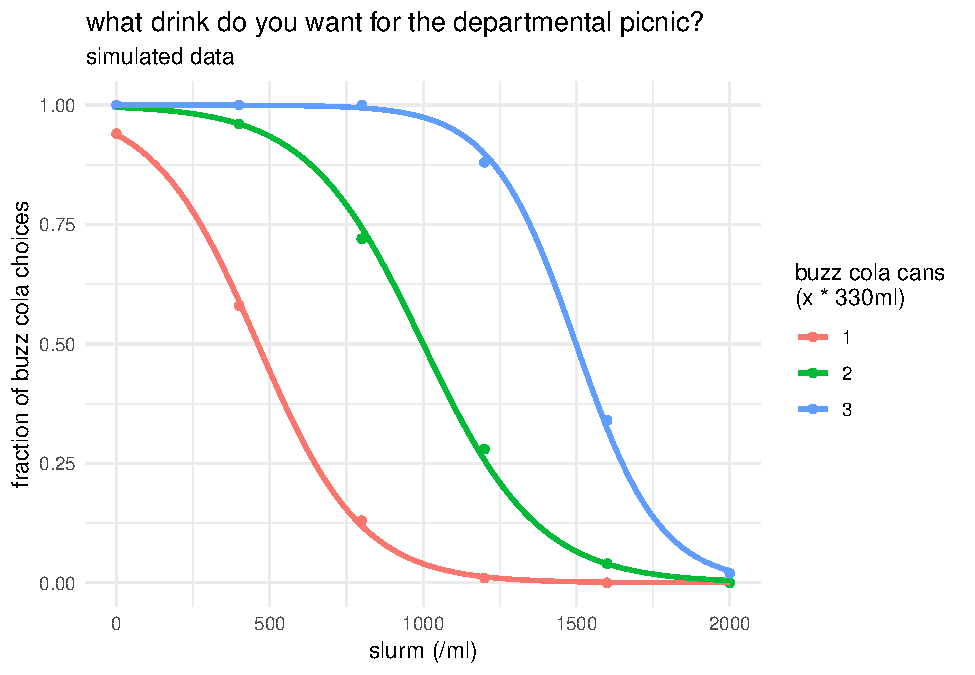
\includegraphics{random_utility_stuff_files/figure-latex/plot_data-1.pdf}

We then need to solve your utilities of buzz cola and slurm. To do this
we need to maximise the sum of the log likelihood of each choice you
make.

Basically, for each trial when you are presented with x ml of buzz cola
(the number of cans multiplied by 330ml per can) or y ml of slurm there
are utility parameters (rho) for both of these which mean you have some
total utility of offered buzz cola and total utility of offered slurm.

As a rational econ PhD student, you are pretty much always going to
choose whichever of these utilities is greater. E.g:

\begin{Shaded}
\begin{Highlighting}[]
\CommentTok{#make up some utility parameters}
\NormalTok{buzz_cola_rho <-}\StringTok{ }\DecValTok{2}
\NormalTok{slurm_rho <-}\StringTok{ }\DecValTok{1}

\NormalTok{trial_utilities <-}\StringTok{ }\NormalTok{trial_data }\OperatorTok
\StringTok{  }\CommentTok{#total utility of each offer is the amount * utility_parameter}
\StringTok{  }\KeywordTok{mutate}\NormalTok{(}\DataTypeTok{buzz_cola_utility =}\NormalTok{ buzz_cola }\OperatorTok{*}\StringTok{ }\DecValTok{330} \OperatorTok{*}\StringTok{ }\NormalTok{buzz_cola_rho,}
         \DataTypeTok{slurm_utility =}\NormalTok{ slurm }\OperatorTok{*}\StringTok{ }\NormalTok{slurm_rho) }\OperatorTok
\StringTok{  }\CommentTok{#which utility is greater}
\StringTok{  }\KeywordTok{mutate}\NormalTok{(}\DataTypeTok{greater_utility =} \KeywordTok{case_when}\NormalTok{(}
\NormalTok{    buzz_cola_utility }\OperatorTok{>=}\StringTok{ }\NormalTok{slurm_utility }\OperatorTok{~}\StringTok{ "buzz_cola"}\NormalTok{,}
\NormalTok{    slurm_utility }\OperatorTok{>}\StringTok{ }\NormalTok{buzz_cola_utility }\OperatorTok{~}\StringTok{ "slurm"}
\NormalTok{  )) }\OperatorTok
\StringTok{  }\CommentTok{#organise columns}
\StringTok{  }\KeywordTok{select}\NormalTok{(buzz_cola, buzz_cola_utility, }
\NormalTok{         slurm, slurm_utility,}
\NormalTok{         greater_utility, choice)}

\CommentTok{#print first 10 trials}
\NormalTok{trial_utilities[}\DecValTok{1}\OperatorTok{:}\DecValTok{10}\NormalTok{,]}
\end{Highlighting}
\end{Shaded}

\begin{verbatim}
##    buzz_cola buzz_cola_utility slurm slurm_utility greater_utility
## 1          3              1980   800           800       buzz_cola
## 2          1               660   800           800           slurm
## 3          1               660   800           800           slurm
## 4          3              1980   800           800       buzz_cola
## 5          3              1980  1200          1200       buzz_cola
## 6          1               660     0             0       buzz_cola
## 7          3              1980   800           800       buzz_cola
## 8          2              1320  1600          1600           slurm
## 9          2              1320     0             0       buzz_cola
## 10         1               660   800           800           slurm
##       choice
## 1  buzz_cola
## 2      slurm
## 3  buzz_cola
## 4  buzz_cola
## 5  buzz_cola
## 6  buzz_cola
## 7  buzz_cola
## 8      slurm
## 9  buzz_cola
## 10     slurm
\end{verbatim}

It's clear to see that mostly the choices fall in line with these made
up parameters. The two unexpected choices could be because of random
participant mistakes, but is more likely due to our paramaters not yet
being optimised (more on that in a sec), or because even rational actors
may sometimes choose something which seems to have less utility
(e.g.~when sampling, or as utilities change e.g.~via satiety).

In the above example, given the relative utilities of the two offered
drinks, it's possible to work out the probability that the participant
will choose either of them using a simple logit model. (for these
formulae I'm copying the notation from
\href{https://imai.fas.harvard.edu/teaching/files/discrete.pdf}{here}).

we have a binary model such that the choice of buzz cola can be
represented by Y: \[Y_{i} \in {0,1}\]

Where X is the difference in utility between the choices A (buzz cola)
and B (slurm) on each trial, i

\[X_{i} = u(A_{i}) - u(B_{i})\] using a logit model such that

\[\phi_{i} = \frac{1}{1 + e^{-\beta X_{i})}}\] where beta is the
temperature of the logit curve (i.e.~the steepness).

The log probability of chossing A (buzz cola) is therefore the log(phi)
when A is chosen, and log(1-phi) when B (slurm) is chosen. The Y/1-Y
cancel the other term out as Y can either equal 1 (buzz cola choice) or
0 (slurm chosen).

We want to sum this over every trial and find the parameters for beta
and the rho for both goods A (buzz cola) and B (slurm) which maximise
this total sum

\[\mathcal l_{n}(\beta|Y,X) = \sum_{i=1}^{n} Y_{i} log(\phi_{i}) + (1-Y_{i})log(1-\phi_{i})\]
In R this can be expressed as

\begin{Shaded}
\begin{Highlighting}[]
\CommentTok{#function to calulate the log likelihood per trial over data}
\CommentTok{#parameters is a vector of beta,rho_a,rho_b}
\CommentTok{#(a = buzz cola, b = slurm)}
\CommentTok{#data is our trial data}
\NormalTok{log_likelihood_func <-}\StringTok{ }\ControlFlowTok{function}\NormalTok{(parameters, data) \{}
  \CommentTok{#I want to plot how optim works so will gather the parameters}
  \CommentTok{#it selects for each iteration}
\NormalTok{  i <<-}\StringTok{ }\NormalTok{i }\OperatorTok{+}\StringTok{ }\DecValTok{1}
\NormalTok{  vals[[i]] <<-}\StringTok{ }\NormalTok{parameters}
  
  \CommentTok{#pull the individual parameters out of the vector}
\NormalTok{  beta <-}\StringTok{ }\NormalTok{parameters[}\StringTok{"beta"}\NormalTok{]}
\NormalTok{  buzz_cola_rho <-}\StringTok{ }\NormalTok{parameters[}\StringTok{"rho_a"}\NormalTok{]}
\NormalTok{  slurm_rho <-}\StringTok{ }\NormalTok{parameters[}\StringTok{"rho_b"}\NormalTok{]}
  
  \CommentTok{#find the trial utility of the offered buzz cola and slurm}
\NormalTok{  trial_bc_utility <-}\StringTok{ }\NormalTok{(data}\OperatorTok{$}\NormalTok{buzz_cola }\OperatorTok{*}\StringTok{ }\DecValTok{330}\NormalTok{) }\OperatorTok{/}\StringTok{ }\DecValTok{1000} \OperatorTok{*}\StringTok{ }\NormalTok{buzz_cola_rho}
\NormalTok{  trial_s_utility <-}\StringTok{ }\NormalTok{(data}\OperatorTok{$}\NormalTok{slurm}\OperatorTok{/}\StringTok{ }\DecValTok{1000}\NormalTok{) }\OperatorTok{*}\StringTok{ }\NormalTok{slurm_rho}
  \CommentTok{#find the difference in utility between the two offered goods}
\NormalTok{  delta_utility <-}\StringTok{ }\NormalTok{trial_bc_utility }\OperatorTok{-}\StringTok{ }\NormalTok{trial_s_utility}
  
  \CommentTok{#find the phi term for this trial}
  \CommentTok{#using the logit model}
\NormalTok{  phi <-}\StringTok{ }\DecValTok{1} \OperatorTok{/}\StringTok{ }\NormalTok{(}\DecValTok{1} \OperatorTok{+}\StringTok{ }\KeywordTok{exp}\NormalTok{(}\OperatorTok{-}\NormalTok{beta}\OperatorTok{*}\NormalTok{delta_utility))}
  
  \CommentTok{#find the log likelihood for the choice made in each trial}
\NormalTok{  log_likelihood <-}\StringTok{ }\NormalTok{(data}\OperatorTok{$}\NormalTok{buzz_cola_choice }\OperatorTok{*}\StringTok{ }\KeywordTok{log}\NormalTok{(phi)) }\OperatorTok{+}\StringTok{ }\NormalTok{((}\DecValTok{1}\OperatorTok{-}\NormalTok{data}\OperatorTok{$}\NormalTok{buzz_cola_choice) }\OperatorTok{*}\StringTok{ }\KeywordTok{log}\NormalTok{(}\DecValTok{1}\OperatorTok{-}\NormalTok{phi))}
  
\NormalTok{  sumloglik[[i]] <<-}\StringTok{ }\KeywordTok{sum}\NormalTok{(log_likelihood)}
  
  \CommentTok{#return the sum over every trial of these log likelihoods}
  \CommentTok{#we want to vary the parameters to maximise this sum}
  \KeywordTok{return}\NormalTok{(}\KeywordTok{sum}\NormalTok{(log_likelihood))}
\NormalTok{\}}
\end{Highlighting}
\end{Shaded}

We can start out with a parameter assuming the two utilities are equal

\begin{Shaded}
\begin{Highlighting}[]
\NormalTok{initial_parameters <-}\StringTok{ }\KeywordTok{c}\NormalTok{(}\DecValTok{1}\NormalTok{, }\DecValTok{1}\NormalTok{, }\DecValTok{1}\NormalTok{) }\OperatorTok
\StringTok{  `}\DataTypeTok{names<-}\StringTok{`}\NormalTok{(}\KeywordTok{c}\NormalTok{(}\StringTok{"beta"}\NormalTok{, }\StringTok{"rho_a"}\NormalTok{, }\StringTok{"rho_b"}\NormalTok{))}

\NormalTok{initial_parameters}
\end{Highlighting}
\end{Shaded}

\begin{verbatim}
##  beta rho_a rho_b 
##     1     1     1
\end{verbatim}

then we can use the optim function which will pass the parameter vector
into the log likelihood funtion and iteratively change the values in the
parameter vector until the greatest sum is returned. We're looking for
the greatest sum as the log likelihood per trial boils down to log(phi /
1-phi) where phi is between 0 and 1 and is greatest where the utility
parameters make the post-hoc choice most clear. E.g. when choosing the
buzz cola the log likelihood = log(phi) and we want to maximise phi.

Taking the log of x between 0 and 1 will give a negative number that
approaches 0 as x approaches 1. So the total sum of log likelihood terms
will approach 0 as the parameters maximise the phi term.

\begin{Shaded}
\begin{Highlighting}[]
\NormalTok{trial_data_binary <-}\StringTok{ }\NormalTok{trial_data }\OperatorTok
\StringTok{  }\KeywordTok{mutate}\NormalTok{(}\DataTypeTok{buzz_cola_choice =} \KeywordTok{case_when}\NormalTok{(}
\NormalTok{    choice }\OperatorTok{==}\StringTok{ "buzz_cola"} \OperatorTok{~}\StringTok{ }\DecValTok{1}\NormalTok{,}
\NormalTok{    choice }\OperatorTok{==}\StringTok{ "slurm"} \OperatorTok{~}\StringTok{ }\DecValTok{0}
\NormalTok{  ))}

\CommentTok{#initialise a list to store the parameters over iterations}
\NormalTok{i <-}\StringTok{ }\DecValTok{0}
\NormalTok{vals <-}\StringTok{ }\KeywordTok{list}\NormalTok{()}
\NormalTok{sumloglik <-}\StringTok{ }\KeywordTok{list}\NormalTok{()}

\NormalTok{optim_params <-}\StringTok{ }\KeywordTok{optim}\NormalTok{(}\DataTypeTok{par =}\NormalTok{ initial_parameters,}
                      \CommentTok{#the functionise to optimise these over}
                      \DataTypeTok{fn =}\NormalTok{ log_likelihood_func,}
                      \CommentTok{#other arguments to the function}
                      \DataTypeTok{data =}\NormalTok{ trial_data_binary,}
                      \CommentTok{#optimisation algorithm to use}
                      \DataTypeTok{method =} \StringTok{"Nelder-Mead"}\NormalTok{,}
                      \CommentTok{#we are looking to maximise the sum}
                      \CommentTok{#so fnscale set to -1}
                      \DataTypeTok{control =} \KeywordTok{list}\NormalTok{(}\DataTypeTok{fnscale =} \OperatorTok{-}\DecValTok{1}\NormalTok{))}
\end{Highlighting}
\end{Shaded}

optim() works by taking a vector of parameters and slightly adjusting
them every iteration until the output from fn = \ldots{} is minimised
via an algorithm (in this case
\href{https://en.wikipedia.org/wiki/Nelder\%E2\%80\%93Mead_method}{Nelder-Mead}).

By collecting the parmater values it selects and the subsequent log
likelihood sum for each iteration we can get a sense of how it works

\begin{Shaded}
\begin{Highlighting}[]
\CommentTok{#load gganimate}
\KeywordTok{library}\NormalTok{(gganimate)}

\CommentTok{#rbind the values per iteration}
\NormalTok{p2 <-}\StringTok{ }\NormalTok{vals }\OperatorTok
\StringTok{  }\KeywordTok{do.call}\NormalTok{(rbind, .) }\OperatorTok
\StringTok{  }\CommentTok{#add a column for iteration number}
\StringTok{  }\KeywordTok{as.data.frame}\NormalTok{() }\OperatorTok
\StringTok{  }\KeywordTok{mutate}\NormalTok{(}\DataTypeTok{iteration =} \DecValTok{1}\OperatorTok{:}\KeywordTok{n}\NormalTok{()) }\OperatorTok
\StringTok{  }\CommentTok{#gather for plotting}
\StringTok{  }\KeywordTok{gather}\NormalTok{(}\StringTok{"parameter"}\NormalTok{, }\StringTok{"value"}\NormalTok{, }\OperatorTok{-}\NormalTok{iteration) }\OperatorTok
\StringTok{  }\CommentTok{#plt a bar chart of parameters over iterations}
\StringTok{  }\KeywordTok{ggplot}\NormalTok{(., }\KeywordTok{aes}\NormalTok{(}\DataTypeTok{x =}\NormalTok{ parameter, }\DataTypeTok{y =}\NormalTok{ value)) }\OperatorTok{+}
\StringTok{  }\KeywordTok{geom_bar}\NormalTok{(}\DataTypeTok{stat =} \StringTok{"identity"}\NormalTok{) }\OperatorTok{+}
\StringTok{  }\CommentTok{#show the iteration in the title}
\StringTok{  }\KeywordTok{labs}\NormalTok{(}\DataTypeTok{title =} \StringTok{'iteration: \{frame_time\}'}\NormalTok{) }\OperatorTok{+}
\StringTok{  }\CommentTok{#aesthetics}
\StringTok{  }\KeywordTok{theme_minimal}\NormalTok{() }\OperatorTok{+}
\StringTok{  }\CommentTok{#gganimate}
\StringTok{  }\KeywordTok{transition_time}\NormalTok{(iteration) }\OperatorTok{+}
\StringTok{  }\KeywordTok{ease_aes}\NormalTok{(}\StringTok{'cubic-in-out'}\NormalTok{)}

\NormalTok{p2}
\end{Highlighting}
\end{Shaded}

\begin{Shaded}
\begin{Highlighting}[]
\NormalTok{p3 <-}\StringTok{ }\KeywordTok{unlist}\NormalTok{(sumloglik) }\OperatorTok
\StringTok{  }\KeywordTok{data.frame}\NormalTok{(}\DataTypeTok{sum =}\NormalTok{ .,}
             \DataTypeTok{iteration =} \DecValTok{1}\OperatorTok{:}\KeywordTok{length}\NormalTok{(.)) }\OperatorTok
\StringTok{  }\KeywordTok{ggplot}\NormalTok{(., }\KeywordTok{aes}\NormalTok{(}\DataTypeTok{x =}\NormalTok{ iteration, }\DataTypeTok{y =}\NormalTok{ sum)) }\OperatorTok{+}
\StringTok{  }\KeywordTok{geom_line}\NormalTok{() }\OperatorTok{+}
\StringTok{  }\KeywordTok{labs}\NormalTok{(}\DataTypeTok{title =} \StringTok{"how optim maximises the sum of the log likelihood"}\NormalTok{,}
       \DataTypeTok{x =} \StringTok{"iteration"}\NormalTok{,}
       \DataTypeTok{y =} \StringTok{"sum of the log likelihoods per trial"}\NormalTok{) }\OperatorTok{+}
\StringTok{  }\KeywordTok{theme_minimal}\NormalTok{()}
\end{Highlighting}
\end{Shaded}

The final maximised value of -400 is still some way off 0 but seems to
be the highest it will go. Looking at p1, we can see that the curves are
some way off a step function that would mean that no `sub-optimal'
choices would be made (there's some threshold of slurm vs buzz cola that
means only one or the other is chosen).

We can then get the optimised paramters from the object returned from
optimisation function

\begin{Shaded}
\begin{Highlighting}[]
\CommentTok{#print the optimised parameters}
\NormalTok{optim_params}\OperatorTok{$}\NormalTok{par}
\end{Highlighting}
\end{Shaded}

and there we have it! you \emph{do} prefer buzz cola (rho\_a) to slurm
(rho\_b)

\subsubsection{You didn't actually solve the
problem}\label{you-didnt-actually-solve-the-problem}

You're right, while we've now collected the parameters for your utility
function in choosing between the two sodas, we now need to ration out
the remaining drinks.

Let's say there are 5 PhDs students (yourself included) left at the
picnic.

\begin{Shaded}
\begin{Highlighting}[]
\KeywordTok{library}\NormalTok{(babynames)}

\NormalTok{names <-}\StringTok{ }\NormalTok{babynames }\OperatorTok
\StringTok{  }\NormalTok{.[}\KeywordTok{sample}\NormalTok{(}\KeywordTok{nrow}\NormalTok{(.), }\DecValTok{5}\NormalTok{),] }\OperatorTok
\StringTok{  }\NormalTok{.}\OperatorTok{$}\NormalTok{name}

\NormalTok{names}
\end{Highlighting}
\end{Shaded}

\begin{verbatim}
## [1] "Kristabelle" "Schaeffer"   "Marius"      "Coletta"     "Lanee"
\end{verbatim}


\end{document}
